% Document settings
\documentclass[11pt]{article}
% % % % % % % % % % % Define Footer
\usepackage{fancyhdr}
\usepackage[margin=1in]{geometry}
\usepackage[pdftex]{graphicx}
\usepackage{multirow}
\usepackage{setspace}
\usepackage{xcolor}
\pagestyle{plain}
\usepackage[american voltages,oldvoltagedirection]{circuitikz}
%\usepackage[american]{circuitikz}
\usepackage{graphicx}
\usepackage{multirow}
\usepackage{booktabs}
\usepackage{epstopdf}
%\usepackage{MnSymbol,wasysym}
\usepackage{amsmath}
%\usepackage{mathtools}
\usepackage{amssymb}
\usepackage{lipsum}
\usepackage{siunitx}
\setlength\parindent{0pt}
\graphicspath{{images/}{drawings/}}
\usepackage{float}
% % % % % % % % % % % Header footer
% % % % % % % % % % %EDIT THIS % % % % % % % % % % % % % % % % % % % %
\pagestyle{fancy}
\fancyhf{}
\lhead{Tech Memo: Experiment 3-Th\'evenin's Equivalent Circuit}
\rhead{Andrei Tumbar}
\lfoot{EE281}
\cfoot{Date }
\rfoot{Page \thepage}
% % % % % % % % % % % % % % % % % % % % % % % % % % % % % % % % % % % % %

\begin{document}
		\numberwithin{equation}{subsection}
		\numberwithin{figure}{subsection}
	\hspace{6in}
		
\includegraphics[scale=0.9,trim=0cm 0in 0in 0.0in,clip]{RIT_KGCOE1}
\newline

\Huge \textbf{EEEE 281 Experiment 3:\\ Th\'evenin's Equivalent Circuit}\\

\Large
\textbf{From:} Andrei Tumbar [Computer Engineering] \\
\textbf{To: } Section 2 TA: LJ Boone, Harrison Keats \\
\textbf{Date: } Performed: 3/3/20  Due: 3/17/20 \\
\textbf{Subject: } Lab 3-Th\'evenin Equivalent Circuits\\
\textbf{Lab Partner(s): } N/A\\
\vspace{0.5in}
	\begin{table}[h!]
		\centering
		%\caption{Grading Table}
		%\label{Table:Grading Table 1}
		%\begin{tabular}{llllll}
		\begin{tabular}{|l||l|l|l|l|}
			\hline
			Component & Percentage of Grade   & Score \hspace{0.5in} & Comment \hspace{0.5in}  \\
			\hline
			Report Formatting & 20~\si{\percent} & & \\	 
			\hline
			\hline 
%			Hand Calculations & 10~\si{\percent} &10 &\colorbox{yellow}{All students get credit.} \\	 	 
%			 \hline
			PSPICE: Setup Conditions & 5~\si{\percent} & & \\	 
			 \hline
			PSPICE: Data and Figures & 15~\si{\percent} & & \\	 
			 \hline
			PSPICE: Discussion of Simulation & 15~\si{\percent} & & \\	 
			\hline
			\hline
			Hardware: Experimental Setup & 10~\si{\percent} & & \\	 
			\hline
			Hardware: Experimental Data and Tables & 15~\si{\percent} & & \\	 
			\hline
			Hardware: Discussion of Results & 20~\si{\percent} & & \\	 
			\hline
			\hline
			\textbf{Total Score:}&  & & \\	 
			\hline
			\textbf{Graded By:}&  & & \\	 
			\hline
		\end{tabular}
	\end{table}
\newpage
\section*{Abstract}
%\Large \textbf{Abstract} \\
\normalsize
%The abstract section should contain a summary of what was performed in the lab and should be approximately  200 words.  This should succinctly rephrase the purpose of the laboratory.  It should also refer to the data collected.    \textbf{The abstract should specifically mentioned the Th\'evenin resistance and voltage obtained, as well as the various methods used.}

This laboratory exercise created a complex circuit were a Thevenin voltage and resistance was determined. To determine the equivalent voltage, a break was placed across the load resistor and the voltage was measured. The equivalent resistance was found by removing independent sources and placing a test source. The current through the test source will indicate the equivalent resistance in the Thevenin circuit. The ammeter in the multimeter was used to measure this current while the volt-meter was used to measure the break voltage.

\section {Introduction and Theory}

%Include 1-2 paragraphs that explains the scope of the experiment. Briefly introduce the concept of Th\'evenin's equivalent circuit.  What was the primary purpose of the experiment? If the data collection has deviated in any way from the rest of your section (for example you had to come back to collect more data), explain this in a second paragraph.  In particular, be sure to note if your data was acquired from a different lab than your classmates/using different equipment. 

The scope of this experiment was to find the equivalent Thevenin circuit by measuring the break voltage and the current through a test source. A Thevenin circuit is one consisting of a voltage source and a resistor. According to Thevenin law, this circuit can represent any complex circuit with any configuration of current or voltage sources whether they be dependent or independent.

\subsection{Theory: Circuit Topology}
%In this section, you should introduce the reader to the circuit  investigated in the experiment, and demonstrate the theoretical value of the circuits. 

%\begin{itemize}
%	\item A figure of the circuit schematic should be included here.  You can use a figure from PSPICE. Be sure to indicate what the load resistor is.  Students using \LaTeX  may ask Dr. Rommel permission to use the Circuitikz artwork used in the laboratory handout. Use of the artwork should be appropriately acknowledged as a citation and under the acknowledgements. If you do use Circuitikz, please let Dr. Rommel know what version you are using.  Some recent updates (discovered while writing this handout/tempalte) have changed the way voltage polarity is presented.  You will hae to edit the values of the resistors. 
%	\item Define the ground in the circuit and specific nodes. 
%	\item This description can be short (a few sentences in length).
%\end{itemize}

The circuit in question is one consisting of seven resistors. A list of parameters controls the value of each resistor. Four different variations of the circuit were designed to gain proper measurements in the simulations.

\begin{figure}[h!]
\begin{center}
\begin{circuitikz}

\draw (0,4) to[battery, *-*, l_=$12\,\si\volt$] (0,0)
	  (0,4) coordinate(A)
	  -- ++(0,1.5) to[R, *-*, a^=$R_1$,l_=$1.0\,k\si\ohm$] ++(8,0) coordinate (B)
	  (A) to[R, *-*, a^=$R_2$,l_=$1.0\,k\si\ohm$] ++(4,0)
	  coordinate (C1)
	  
	  to[R, *-*, a^=$R_3$,l_=$1.0\,k\si\ohm$] ++(4,0) coordinate(C)
	  
	  (B) -- (C)
	  to[R, *-*, a^=$R_L$,l_=$5.6\,k\si\ohm$] ++(0,-4)
	  to[R, *-*, a^=$R_5$,l_=$1.0\,k\si\ohm$] ++(-4,0) coordinate(D)
	  to[R, *-*, a^=$R_4$,l_=$1.0\,k\si\ohm$] ++(-4,0)
	  (C1) to[R, *-*, a^=$R_6$,l_=$10\,k\si\ohm$] (D)
	  
	  (0,0) node[ground]{};

\end{circuitikz}
\label{fig:circuit}

\caption{Circuit showing the ground, power-source, and load configuration}

\end{center}
\end{figure}

Figure \ref{fig:circuit} depicts the circuit in question. All resistors are $1.0\,k\si\ohm$ with the exception of $R_6$ which is $10\,k\si\ohm$ and the load resistor, $R_L$, is $5.6\,k\si\ohm$. A $12\,\si\volt$ power source is connected to power the circuit.

%\subsection{Theory: Hand Calculations and PSPICE of Th\'evenin Equivalent Circuit}
%\colorbox{yellow}{\textcolor{blue}{Hand calculations are \textbf{not} required for this lab report.}}
%
\subsection{Theory: PSPICE Simulation Summary}
%Begin by providing a 1 paragraph description of the PSPICE setup.  Which \textbf{libraries} and \textbf{PSPICE elements} were used in the simulation? You can borrow from the text of your first tech memo here.  If you do so, please be sure to cite the tech memo. Note the libraries used. You can find the information when you look at the properties of each element.  There will be a reference to a ``.olb'' file.  This is the library name. 

The PSPICE simulation began with a design of the circuit. The PSPICE setup used the libraries imported from the Circuits 1 library from the lab computer. The libraries were called \textbf{analog.olb}, \textbf{opamp.olb}, \textbf{source.olb}, and \textbf{special.olb}. The components used were ``R/ANALOG'' from the \textbf{analog.olb} for the resistors, ``VDC/SOURCE'' from the \textbf{source.olb} for the voltage source and ``O/CAPSYM'' and ``PARAMETER/SPECIAL'' from the \textbf{special.olb} for ground.

%Include a description of the resistor sweep.  Specifically, what is the function of the \textbf{PARAMETER/SPECIAL} element?   Also, what type of simluation was run?What were the start/stop resistor values? What was the step size, and was it linearly or logarithmically varied?    Comment about the line fit in Excel (or whatever software was used to perform the linear regression).

A parameter list using the ``PARAMETER/SPECIAL'' component was used to allow the values of each resistor be easily changed. Rcommon controlled the value of every resistor apart from $R_6$ and $R_L$ A resistor sweep was performed in the PSPICE so that the voltage across $R_L$ could be measured for varying values of $R_L$. The slope of the curve would yield the Thevenin resistance while the intercept would represent the Thevenin voltage.

%The lab handout called for using parameters in the tutorial, which were edited during your prelab to match the resistors in this lab.  What changes were made to the parameters?  Also, why were unique names given for Net Aliases in each circuit?
\subsubsection{Theory: PSPICE Schematic Diagram}
%Since the prelab called for having all 4 circuits on the same page, you may place two copies of the schematic here as listed in Figs. \ref{Fig:SchematicVoltMarkers} and \ref{Fig:SchematicCurrentMarkers}

\begin{figure}[h!]
	\begin{center}
		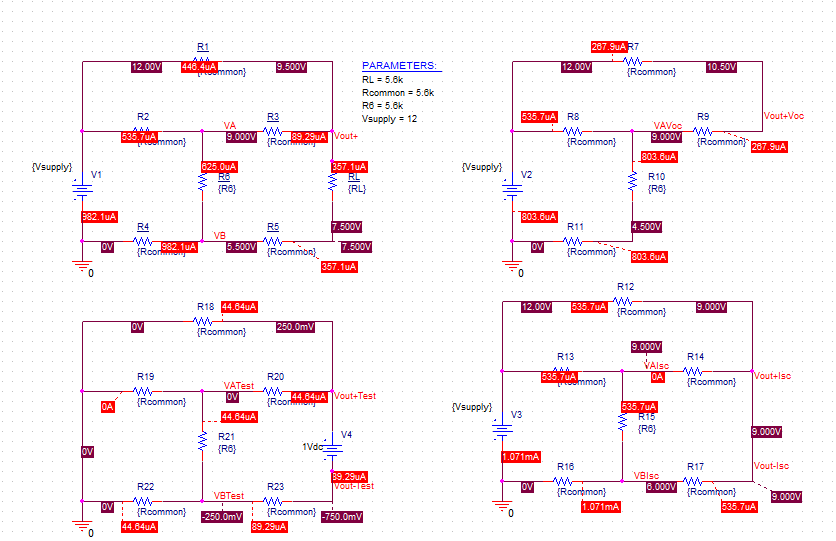
\includegraphics[width=\textwidth]{schematic_1}
		\caption{Screen shot of the PSPICE schematic with voltage markers.}
		\label{Fig:SchematicVoltMarkers}
	\end{center}
\end{figure} 

%Include a brief description of the figures (which subcircuit is which-i.e., The upper right schematic diagram is the Variable Load).

The top left schematic is the full circuit. The top right shows the circuit needed to calculate the Thevenin voltage. A break can be seen where the load resistor was. The bottom left depicts a test source being added to the circuit with all of the independent power sources removed. This is used to find the equivalent resistance of the circuit. The final circuit is one were there is a short across the $R_L$ to measure the current through the point when the resistance is $0\,\si\ohm$.

\subsubsection{Theory: PSPICE Simulation Varying Load Circuit}
 %In this section, include: 

\begin{figure}[h!]
	\begin{center}
		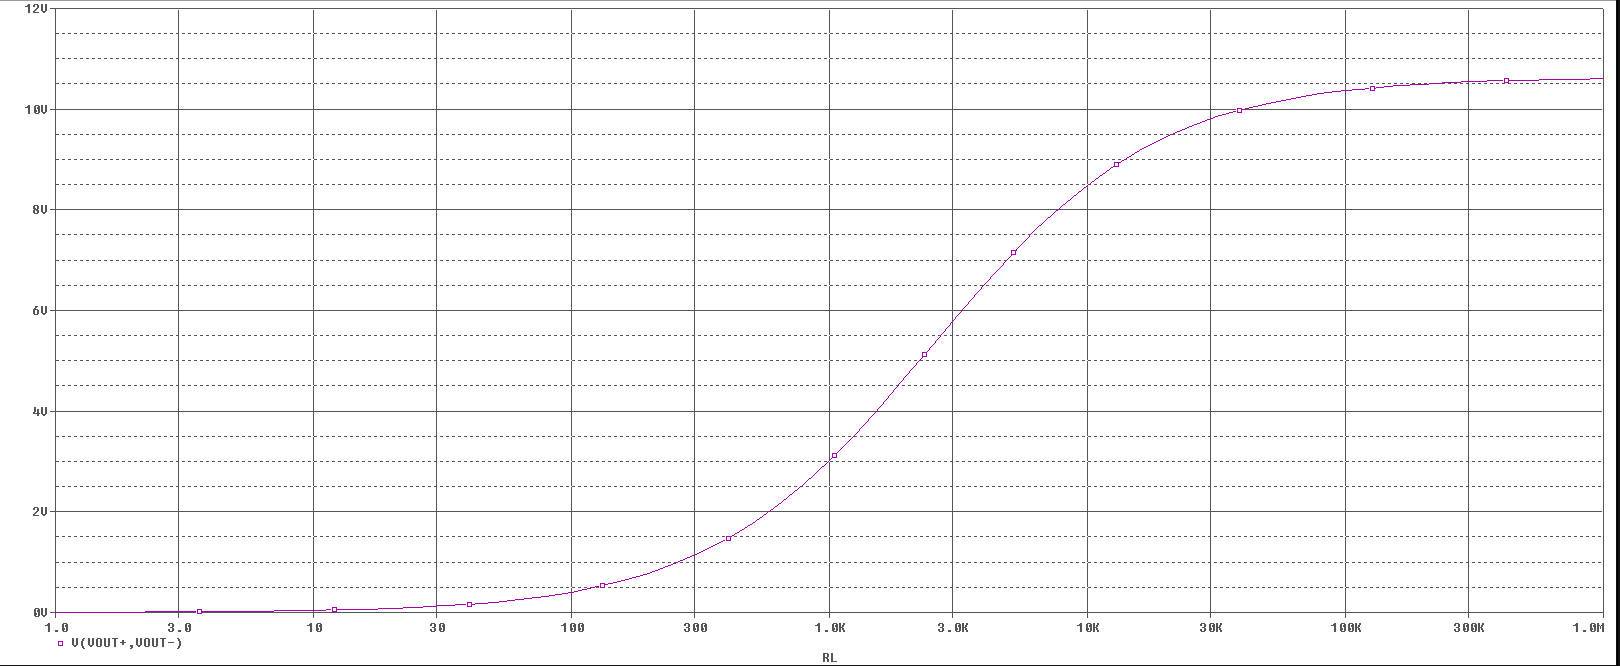
\includegraphics[width=\textwidth]{simulation}
		\caption{Screen shot of the PSPICE resistor sweep simulation.}
		\label{Fig:SimulationSweep}
	\end{center}
\end{figure}

Figure \ref{Fig:SimulationSweep} shows the voltage curve as the resistor sweep simulation was calculated. A number of different resistance values were used to calculate the voltage across $R_L$.\\\\\\

% \begin{itemize}
% 	\item A figure with the plot of $R_L$ vs. $v_{L}$ from PSPICE.
% 	\item A figure with the corresponding linear regression in Excel that illustrates the resulting scatter plot and extraction of $R_{th}$. 
% 	\item Present the equation generated by Excel in the text of the report.
% 	\item Be sure to indicate the $r^2$  value with the equation. You may need to change the output precision of Excel if the $r^2$ value appears to be ``1''.  Realistically simulation results will show a ``1''.
% 	\item Table \ref{Table:Lab3VariableLoadPSPICE} shows the Thevenin voltage and resistance calculated from the excel document. The results agree with that of the tutorial.
\begin{table}[htbp]
	\caption{Variable Load PSPICE test results}.
	\begin{center}
	\label{Table:Lab3VariableLoadPSPICE}
	%\begin{tabular}{llllll}
	\begin{tabular}{|c|c|c|c|}
		\hline
		$V_{th}$ (\si{\volt})& %$I_{sc}$ (\si{\milli\ampere}) &
		 $R_{th}$ (\si{\ohm}) \\
		\hline
		10.629	& 2514.3 \\	 \hline 
	\end{tabular}
	\end{center}
\end{table}

By graphing the voltage vs current, number of qualities about the circuit can be gained from the linear progression that is generated.

\begin{figure}[h!]
	\begin{center}
		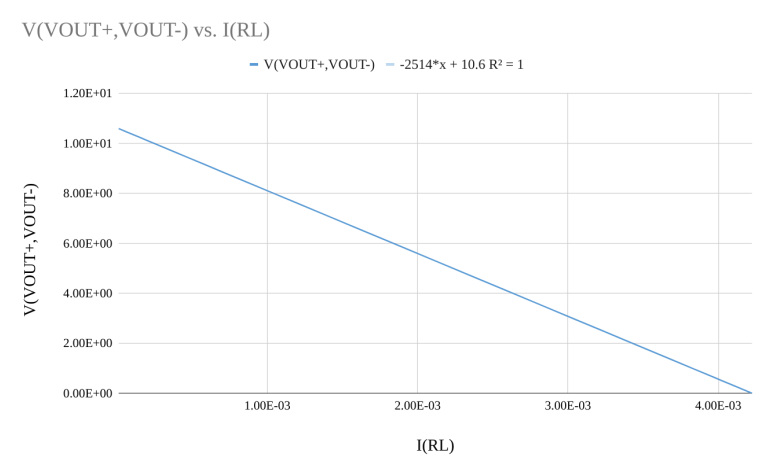
\includegraphics[height=8cm]{regression}
		\caption{Linear regression of $V_L$ vs $R_L$}
		\label{Fig:SimulationRegression}
	\end{center}
\end{figure}

% \end{itemize}

The regression in Figure \ref{Fig:SimulationRegression} shows a line with the equation:

\begin{align}
y=-2514x + 10.6 && R^2 = 1
\end{align}

The align of this line indicates the Thevenin resistance while the Y-intercept is the Thevenin voltage. This is because when the current is zero, the circuit has a break therefore the voltage across $R_L$ is the Thevenin voltage. The slope of the graph is the negative of the Thevenin resistance because we are graphing $V$ vs $-I$ therefore the slope can be seen as $-R = \frac{V}{-I}$.

\subsubsection{Theory: PSPICE Simulation Open Circuit/Short Circuit Test}
 %In this section, include: 
 %\begin{itemize}
% 	\item Explain how the PSPICE schematic was altered for the open circuit voltage test and short circuit test. The entire discussion (including all bullets below) should be about 1 paragraph
% 	\item Refer to the Fig. \ref{Fig:SchematicVoltMarkers} with a screen shot of the schematic in PSPICE with voltage markers for the $V_{oc}$ test.  As you likely have already placed this figure in your theory section, there is no need to do so a second time.  
% 	\item Refer to Fig. \ref{Fig:SchematicCurrentMarkers} with a screen shot of the schematic in PSPICE with current markers for the $I_{sc}$ test.  As you likely have already placed this figure in your theory section, there is no need to do so a second time.

The open circuit test in Figure \ref{Fig:SchematicVoltMarkers} (top-right), is generated by creating a break in the circuit where the load resistor ($R_L$) is found. This also effectively removes $R_5$ as it is in series with this break and therefore no current is passing through it and no voltage drop can be measured across it. In the bottom right of Figure \ref{Fig:SchematicVoltMarkers}, the short circuit test can be seen. Here a wire is placed across $R_L$ and the current is measured through the wire.

\begin{table}[h!]
	\centering
	\caption{PSPICE Open/Short Test Table}.
	\label{Table:Lab3VocIscPSPICE}
	%\begin{tabular}{llllll}
	\begin{tabular}{|c|c|c|c|}
		\hline
		$V_{th}$ (\si{\volt})& $I_{sc}$ (\si{\milli\ampere}) & $R_{th}$ (\si{\ohm}) \\
		\hline
		10.629 & 4.227 & 2515.02 \\	 \hline 
	\end{tabular}
\end{table}
% \end{itemize}
 
Table \ref{Table:Lab3VocIscPSPICE} shows the $R_{th}$ calculations when the voltage across the load is measured with a break and the current through the load is measured with a short. The results agree with the PSPICE simulation.
 
\subsubsection{Theory: PSPICE Simulation Test Signal Method }
%In this section, include: 
%\begin{itemize}
% 	\item Explain how the PSPICE schematic was altered for the open circuit voltage test and short circuit test. The entire discussion (including all bullets below) should be about 1 paragraph
% 	\item Refer to the Fig. \ref{Fig:SchematicCurrentMarkers} with a screen shot of the schematic in PSPICE with current markers for the Test signal.  As you likely have already placed this figure in your theory section, there is no need to do so a second time.  
% 	\item The results in Table \ref{Table:Lab3ReqTestSignalPSPICE} agree with the results from $V_{OC}$ and $I_{SC}$ in the tables about. This table shows the thevenin resulting circuit if a 1V source was added. 

In the bottom left of Figure \ref{Fig:SchematicVoltMarkers} the test signal can be seen. Here the circuit is altered by removing all of the independent sources. Voltage sources become wires and current sources become breaks. The load resistor is replace by a voltage source with a chosen voltage. $1\,\si\volt$ is chosen for this test source.

\begin{table}[h!]
	\centering
	\caption{$R_{th}$ from Test Signal.}
	\label{Table:Lab3ReqTestSignalPSPICE}
	%\begin{tabular}{llllll}
	\begin{tabular}{|c|c|c|c|c|c|}
		\hline
		Test Signal  (\si{\volt}) &$V_{R5}$ (\si{\volt}) & $I_{\mbox{Test Signal}}$ (\si{\milli\ampere}) & $R_{th}$ (\si{\ohm})\\
		\hline
		1.0 & .3977 & 0.3977 & 2514.5 \\	 \hline 
	\end{tabular}
\end{table}

Using the test signal method, the $R_{th}$ value was calculated to be very close to that of the other method. These two measurements agree.

%\end{itemize}

\section{Hardware Experiment: Results and Discussion}
%This section of the report should present what was done in hardware.  A reader should be able to recreate an experiment from the detail present.  One section discusses the equipment used in the experiment. The remaining sections discuss the results for each circuit.

In the hardware portion of this experiment, the Thevenin voltage and Resistance were measured using various methods. A graph was created to mimick the resistor sweep done in PSPICE.

\subsection{Equipment Used in the Laboratory}
%Write a short paragraph to detail the equipment used in the laboratory, and specific model numbers. Ideally, you should create a table of the equipment which should be referred to in text (See Table \ref{Table:Equipment} as an example).  The room location where the experiment was performed should be included.  Note that this should be a part of all Tech Memos, as it is an essential piece for other users to replicate your experiment.  \textbf{As you will be likely using the same equipment throughout the term, once the text/tables are established, you may reuse the information with the permission of your instructor/TA. Again, cite your first lab report as a reference.}

PSPICE Capture CIS was used to create the circuit and the perform the simulation. The DC Power Supply shown in Table \ref{Table:Equipment} was used in the hardware portion to power the circuit. The multimeter shown was used to measure the voltage and resistances across each of the resistors.

\begin{table}[htbp]
	\setlength{\tabcolsep}{14pt}
	\caption{Equipment/Software required for Lab 3.}
	\label{Table:Equipment}
	\begin{center}
	%\begin{tabular}{llllll}
		\begin{tabular}{|c||c|c|c|c|}
			\hline
			Item & Tool & Room      \\
			\hline
			Simulation & OrCAD Capture CIS & 09-3200   \\
			\hline  
			DC Power Supply & Agilent E3631A   & 09-3200 \\ 
			\hline 
			Multimeter & Agilent 34401A & 09-3200 \\
			\hline
			%				Oscilloscope & Textronix TDS2012C & 09-3200  \\
			%				\hline
			%				Oscilloscope & Agilent DSO 33120A & 09-3170  \\
			%				\hline
			%				
		\end{tabular}
	\end{center}
\end{table}

\subsection{Hardware Results/Discsussion Resistor Values}	
%Begin the section by including the experimental values of the resistors as illustrated in Table \ref{Table:Lab3Resistors}. If you kept your lab 2 circuit wired up for lab 3, you can include the table (cut/paste), citing your lab 2 report. Briefly discuss.

Table \ref{Table:Lab3Resistors} shows the experimentally determined resistor values for each of the resistors used in the circuit. All of the resistors were in an acceptable range from the rated $5.6\,k\si\ohm$ value.

  	\begin{table}[h!]
  		\centering
  		\caption{Resistors used in the laboratory.}
  		\label{Table:Lab3Resistors}
  		%\begin{tabular}{llllll}
  		\begin{tabular}{|c||c|c|c|c|}
  			\hline
  			Resistor &Exp. Value (\si{\kilo\ohm})  \\
  			\hline
  			$R_{1}$  & 0.983 \\	 \hline 
  			$R_{2}$  & 0.983 \\	 \hline 
  			$R_{3}$  & 0.987 \\	 \hline 
  			$R_{4}$  & 0.981 \\	 \hline 
  			$R_{5}$  & 0.982 \\	 \hline 
  			$R_{6}$  & 9.95 \\	 \hline
  		\end{tabular}
  	\end{table}

\subsection{Hardware Results: Open/Short Extraction}
  \begin{table}[h!]
  	\centering
  	\caption{Hardware Open/Short Test Table}.
  	\label{Table:Lab3VocIsc}
  	%\begin{tabular}{llllll}
  	\begin{tabular}{|c|c|c|c|}
  		\hline
  		$V_{th}$ (\si{\volt})& $I_{sc}$ (\si{\milli\ampere}) & $R_{th}$ (\si{\ohm}) \\
  		\hline
  		10.475 & 4.547 & 2303.7 \\	 \hline 
  	\end{tabular}
  \end{table}
%  Include the following discussion points in a paragraph:
%  \begin{itemize}
%  	\item A table of the measured open circuit voltage and short circuit current  (Table \ref{Table:Lab3VocIsc}).
%  	\item Provide a discussion of how you implemented the technique in hardware (i.e., What did you change in the hardware circuit to measure the open circuit voltage?  What did you change in the hardware circuit to measure the short circuit current?)
%  	\item For the short circuit current, you most likely extracted this by measuring a voltage across the $R_5$ resistor in the lab handout.  Include the Ohm's law calculation to back out the current as an inline equation. 
%  	\item Discuss how the results agree with theory, and include an error analysis based on either the PSPICE or hand calculations.
%  \end{itemize}

To determine the Thevenin voltage and resistance using the open/short circuit test, the load resistor was removed from the circuits. Using the $12\,\si\volt$ source a multimeter measuring voltage was placed across the load resistor terminals. Next, the fuse on the multimeter was changed to be used as an ammeter. The ammeter terminals were placed inside the nodes where $R_L$ attached. The measured values were recorded in Table \ref{Table:Lab3VocIsc}. A Thevenin resistance was calculated using Ohm's Law. These results agree with the simulation. The value is around $200\,\si\ohm$ lower than the simulated value because most of the experimental resistors were slightely under their rated values.

\subsection{Hardware Results: Direct Measurement of $R_{th}$}
%In this section, discuss the  direct measurement of $R_{th}$ in  1 paragraph.
%\begin{itemize}
%  	\item Provide a discussion of how you implemented the technique in hardware.  What was done to the load resistor? What was done to the power supply?  How was $R_{th}$ measured?
%  	\item Record the value of $R_{th}$ from direct measurement in Table \ref{Table:Lab3RthDirect}.
%  	\item Discuss whether the results agree with theory.
%  \end{itemize}

The direct method of $R_{th}$ is done by shorting the connection between the power source terminals and using the mutlimeter to measure the resistance across the load terminals. \\

\begin{table}[h!]
	\centering
	\caption{$R_{th}$ direct measurement table}
	\label{Table:Lab3RthDirect}
	%\begin{tabular}{llllll}
	\begin{tabular}{|c|c|c|c|}
		\hline
		$R_{th}$ (\si{\kilo\ohm})& $2.360\,k\si\ohm$ \\
		\hline 
	\end{tabular}
\end{table}

Table \ref{Table:Lab3RthDirect} shows the results of the direct measurement. These results agree with the simulation and the open/short circuit test.

\subsection{Hardware Results:  Test Signal Extraction}

The test signal is a method used to determine the Thevenin resistance. By removing the independent sources, only the Thevenin resistor is kept in the circuit and therefore by placing a source of our choosing, the resistance can be determined. The test signal is placed across the load and then the current through the source is determined. To easily find this current, the voltage across the resistor in series with the source can be measured, in this case $R_5$ was used.

%In this section, discuss the  test signal extraction measurement of $R_{th}$ in  1 paragraph.



%\begin{itemize}
%\item Provide a discussion of how you implemented the technique in hardware.  What was done to the load resistor? What was done to the power supply? Where did you hook up the test signal, and what was the magnitude of the test signal? How was $R_{th}$ determined?
%\item Record the value of $R_{th}$ from the test signal extraction in Table \ref{Table:Lab3ReqTestSignal}.
%\item Discuss whether the results agree with theory.
%\item Answer the following question: If the test signal was increase to 3~\si{\volt}, would the final result change? Explain.
%\end{itemize}

\begin{table}[h!]
	\centering
	\caption{$R_{th}$ from Test Signal.}
	\label{Table:Lab3ReqTestSignal}
	%\begin{tabular}{llllll}
	\begin{tabular}{|c|c|c|c|c|c|}
		\hline
		Test Signal  (\si{\volt}) &$V_{R5}$ (\si{\volt}) & $I_{R5}=i_{test}$ (\si{\milli\ampere}) & $R_{th}$ (\si{\ohm})\\
		\hline
		1.0 & 0.426 & 0.426 & 2347.4 \\	 \hline 
	\end{tabular}
\end{table}

A $1\,\si\volt$ test source was used for simplicity. The results shown in Table \ref{Table:Lab3ReqTestSignal} agree with the previous measurements and the simulations. If the test source was changed to $3\,\si\volt$, the results would not change because the current $i_{test}$ would change accordingly which would result in the same $R_{th}$ value to be calculated.

\subsection{Hardware Results: Varying Load Extraction}
%In this section, you should discuss the hardware results of the varying load extraction.  Include the following:

%\begin{itemize}
%\item A table of the measured load voltage, and corresponding load current for each resistor (Table \ref{Table:Lab3LoadResistors}).
%\item A scatter plot of this data  in Excel/Matlab/etc. showing the line fit extraction and corresponding Th\'evenin Resistance.   As described in the prelab video, be sure to indicate the $r^2$  value with the equation. You may need to change the output precision of Excel if the $r^2$ value appears to be ``1''. 
%\item Briefly discuss whether the results compare to the PSPICE theory.
%\end{itemize}

The varying load experiment is similar to the resistor sweep. The load resistor was changed for multiple valued resistors and the voltage across the load was measured. A current was calculated and then graphed.

\begin{table}[htbp]
	\centering
	\caption{Variable load resistor Table.  Use Ohm's Law to determine the load current ($I_L$)}.
	\label{Table:Lab3LoadResistors}
	%\begin{tabular}{llllll}
	\begin{tabular}{|c||c|c|c|c|}
		\hline
		Resistor &Exp. Value (\si{\kilo\ohm}) &$V_{RL}$ (\si{\volt}) & $I_L$ (\si{\ampere}) \\
		\hline
		$R_{L1}$ & 120   & 0.512 & 0.00426 \\	 \hline 
		$R_{L2}$ & 390   & 1.500 & 0.00385 \\	 \hline 
		$R_{L3}$ & 2.20k & 5.101 & 0.00223 \\	 \hline 
		$R_{L4}$ & 4.70k & 7.010 & 0.00149 \\	 \hline 
		$R_{L5}$ & 5.60k & 7.379 & 0.00132 \\	 \hline 
		$R_{L6}$ & 8.20k & 8.160 & 0.000995 \\	 \hline
		$R_{L7}$ & 15.0k & 9.070 & 0.000605 \\	 \hline
		$R_{L8}$ & 18.0k & 9.275 & 0.000515 \\	 \hline 
	\end{tabular}
\end{table}

The values shown in Table \ref{Table:Lab3LoadResistors} where used to generate a graph and a linear regression.
\pagebreak

\begin{figure}[h!]
	\begin{center}
		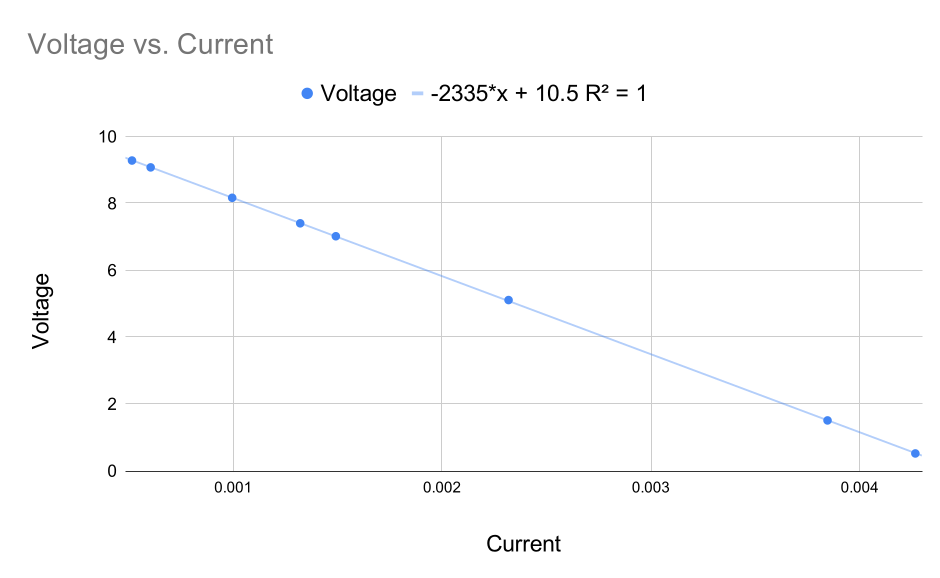
\includegraphics[height=8cm]{volt_vs_current}
		\caption{Linear regression of $V_{RL}$ vs $I_L$}
		\label{Fig:ExperimentRegression}
	\end{center}
\end{figure}

Figure \ref{Fig:ExperimentRegression} is a graph of Table \ref{Table:Lab3LoadResistors} where current is on the X-axis and voltage on the Y. The Y-intercept is the Thevenin voltage because that is where the circuit has a break. The slope of the the line is the measured Thevenin resistance. The value $2335\,\si\ohm$ agrees with the previous experiments and the simulations.

\section{Conclusion}

This laboratory experiment attempted to prove the validity of Thevenin's Theory that any complex circuit could be simplified relative to a load component where the load is in series with a voltage source and a resistor. The lab started with simulations of the circuit in which the voltage across the break of the load was measured as well as the current through the short. Also, a test source was placed instead of a resistor on the load as an alternative method for determining the Thevenin resistance. A resistor sweep was conducted where the voltage across a varying resistor was measured from $1\,\si\ohm$ to $1\,M\si\ohm$. In the hardware portion, the simulations were conducted on a breadboard. A break voltage and short current were measured along with a direct measurement of the Thevenin resistance. A $1\,V$ test source was also used to determine this resistance. Finally, a resistor sweep was conducted where eight different resistors were used as the load elements and the voltage across them were measured and graphed. This laboratory experiment validates Thevenin's Theorem experimentally because the calcuated value is relatively close to the simulated value. The relative different can be attributed to the slight variance from the rated resistance. These differences collectively caused an experimentally determined Thevenin resistance to be around $200\si\ohm$ lower than the simulated resistance.

%Provide a 1 paragraph summary of the laboratory experiment.  What were the major conclusions for each part of the experiment?  Also did the theory agree with the experiment?  The conclusion is a revised version of the abstract.  Has Th\'evenin's Theorem been experimentally validated?  Discuss the effects of tolerances affecting the differences between measured results and simulated results.

\pagebreak
\section{Acknowledgments}

\begin{itemize}
	\item wikibooks.org helped with the \LaTeX\;code.
	\item tex.stackexchange.com helped with the circuit diagram in \LaTeX.
	\item Petre Tumbar and Walter Sigel were present in the lab for the prelab and experiment.
\end{itemize}

%Acknowledge \textbf{any} source of help received in the experiment/writing the report.  This should certainly include your lab partner/teaching assistant/instructor.  It may also include other classmates/study partners. State briefly what the nature of the help was.
	
%\textbf{Your report should include references to appropriate pages in the text, as well as any other sources, websites/etc. consulted in the preparation of the report.}

\begin{thebibliography}{9}
	\bibitem{AlexanderSadiku}
	C.K. Alexander, and M.K.O. Sadiku,
	\emph{Fundamentals of Electric Circuits, 4th Edition},
	McGraw Hill, pp. all slides, 2009.
	\bibitem{OldLab}
A. Tumbar,
	\emph{EEEE 281 Lab 2 Tech Memo},
	all pages, submitted 2, 18, 2020.
	\bibitem{RommelLab}
	S. Rommel,
	\emph{EEEE 281 Lab 3 Lecture notes},
	all slides, Spring 2015.
\end{thebibliography}

\end{document}
